\section{\textit{Layers} de la PCB}
    A continuación se presentan los diseños finales que concluyen el capítulo \ref{ch:CH04} de diseño electrónico concluye con la presentación de los layers y las vistas \ac{CAD} del diseño de la \ac{PCB} de control y de la \ac{PCB} de sensado de velocidad. Sus dimensiones se tomarán como referencia en el Capítulo \ref{ch:CH05}, dedicado al ensamblaje en el chasis. En la Figura \ref{fig:Layers} se muestran las imágenes finales de las tarjetas.
    \begin{figure}[H]
        \begin{tabularx}{\linewidth}{*{2}{>{\centering\arraybackslash}X}}
            % FILA-1, COL-1.
            \begin{subfigure}[t]{0.45\textwidth}
                \centering
                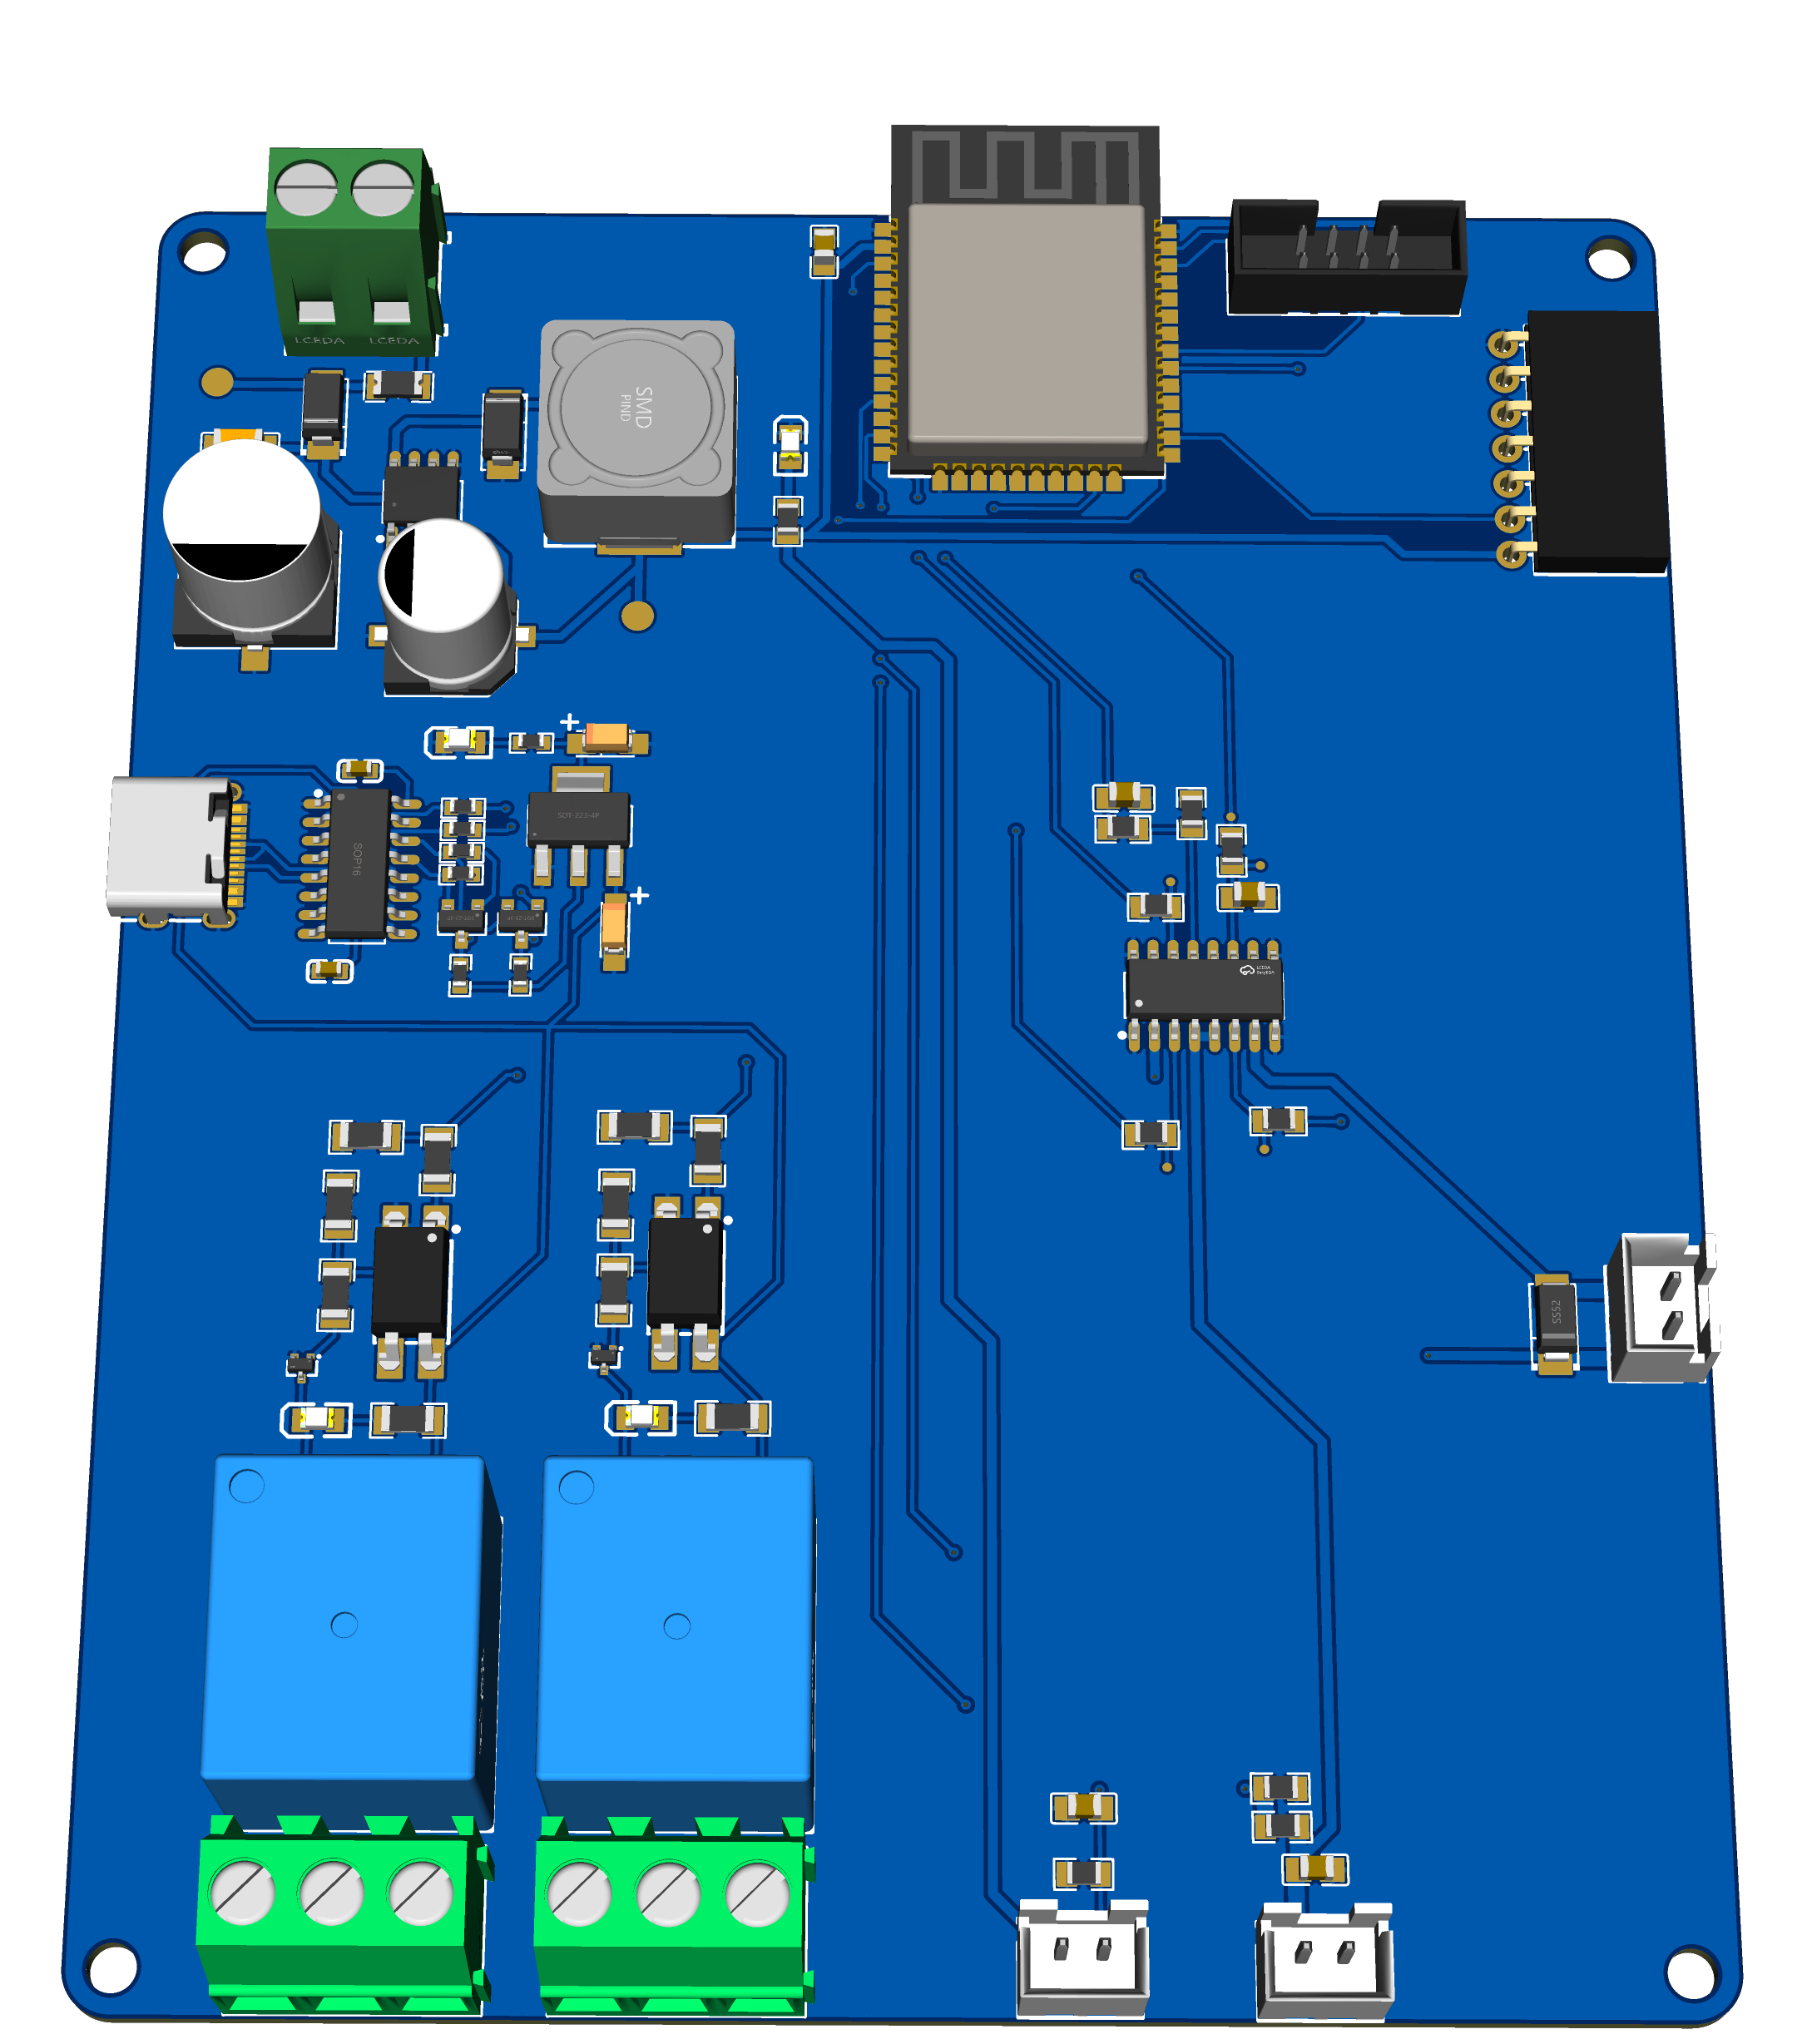
\includegraphics[width=.9\linewidth]{CHPTRS/CH04_DIS_ELECTRONICO/Fig_Esquematicos/3D_PCB10_2026-01-30.png}
                %\label{fig:imagen_pcb_control} %LABEL ESTA DESPUES
            \end{subfigure}
            & %Nueva Columna, es decir: % FILA-1, COL-2
            \begin{subfigure}[t]{0.45\textwidth}
                \centering
                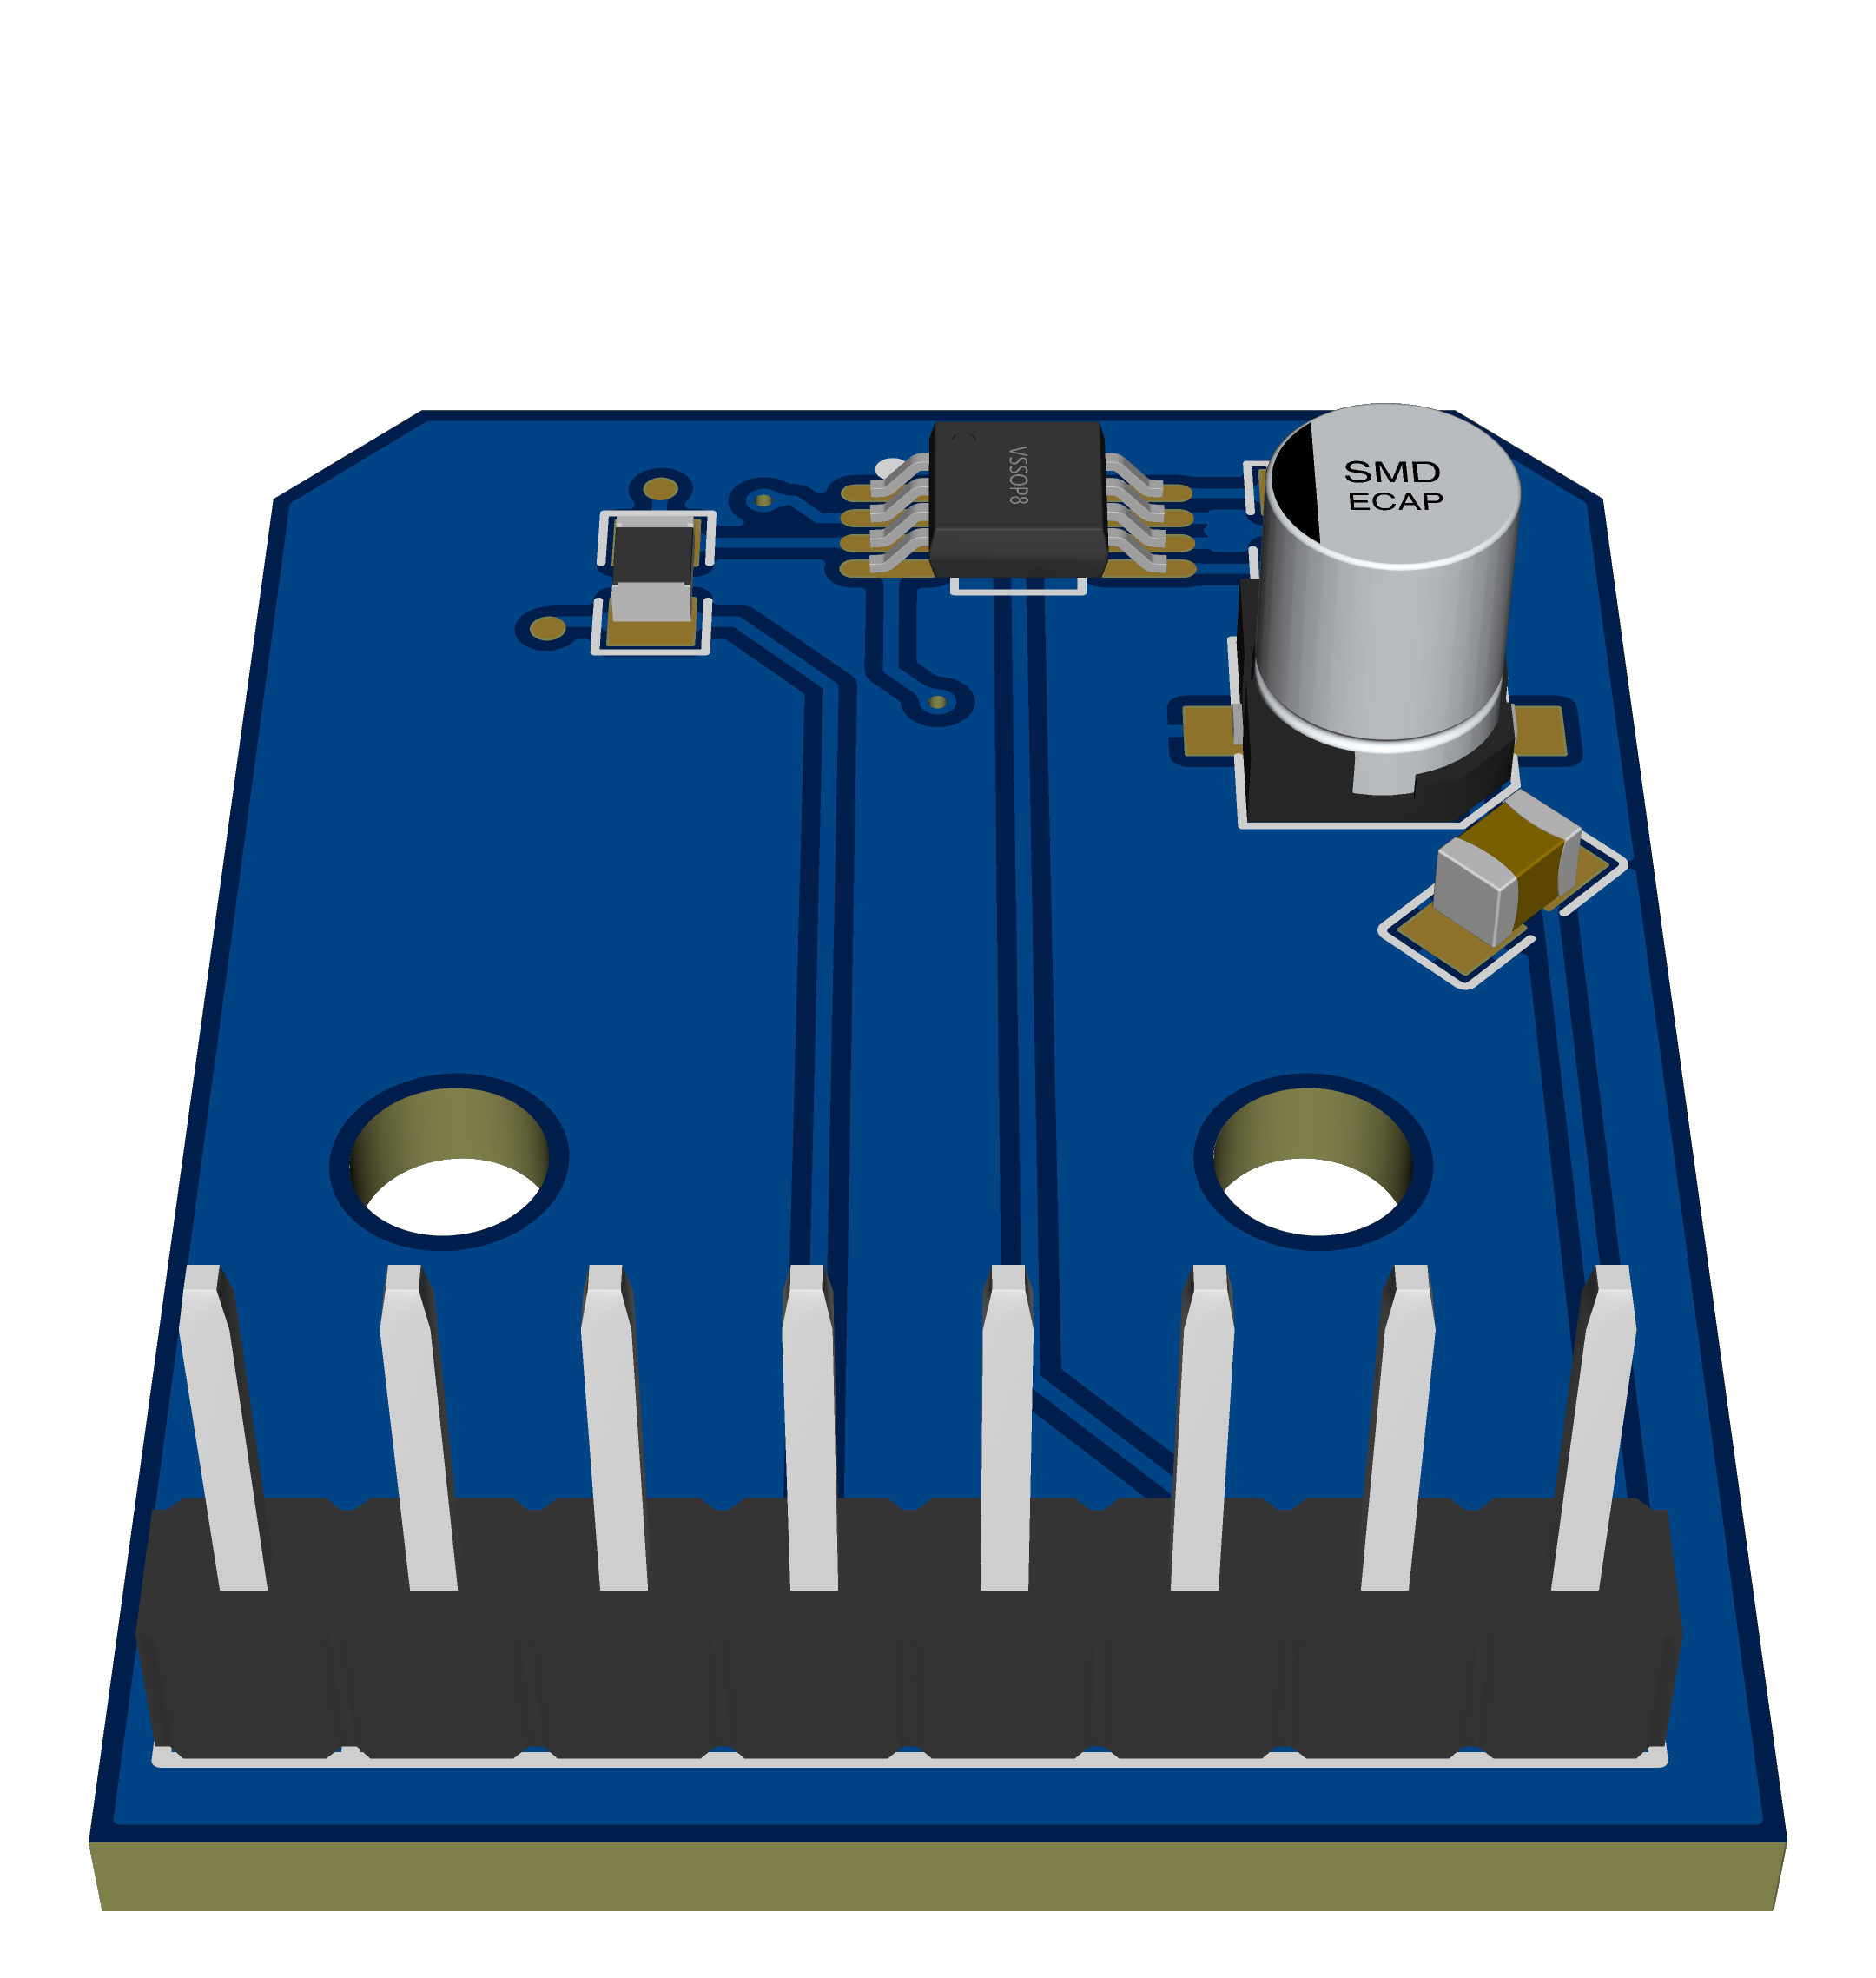
\includegraphics[width=.68\linewidth]{CHPTRS/CH04_DIS_ELECTRONICO/Fig_Esquematicos/PCB_sensor.png}
            \end{subfigure}
            \\ %Nueva Fila, es decir: % FILA-2, COL-1
            \begin{subfigure}[t]{0.8\linewidth}
                \caption{Imagen referencial de cómo quedará la \ac{PCB} de control}
                \label{fig:romeo}
            \end{subfigure} 
            & %Nueva Columna, es decir: % FILA-2, COL-2
            \begin{subfigure}[t]{0.8\linewidth}
                \caption{Imagen referencial de cómo quedará la \ac{PCB} para el sensor de efecto \textit{hall}}
                \label{fig:imagen_pcb_tmag5170}
            \end{subfigure}
        \end{tabularx}
        \caption{Vista general de las \ac{PCB}s de control y la de \textit{encoder}}
        \label{fig:Layers}
    \end{figure}

    En esta sección se presentan los \textit{layers} de las dos tarjetas diseñadas para el sistema: una tarjeta de control, encargada de la gestión de señales y alimentación, y una tarjeta dedicada al sensor de efecto \textit{hall}. Esta última no se monta sobre la tarjeta de control, debido a que debe ubicarse en la zona de pruebas del motor para realizar el sensado directamente sobre el eje.

\subsection{\textit{Layers} de la tarjeta de control}
A continuación se muestran los \textit{layers} de la tarjeta de control: la capa \textit{Top} en la Figura~\ref{fig:ctrl_top} y la capa \textit{Bottom} en la Figura~\ref{fig:ctrl_bottom}, presentadas de forma conjunta en la Figura~\ref{fig:pcb_ctrl_layers}.

\begin{figure}[H]
\centering
\begin{subfigure}[t]{0.4\textwidth}
  \centering
  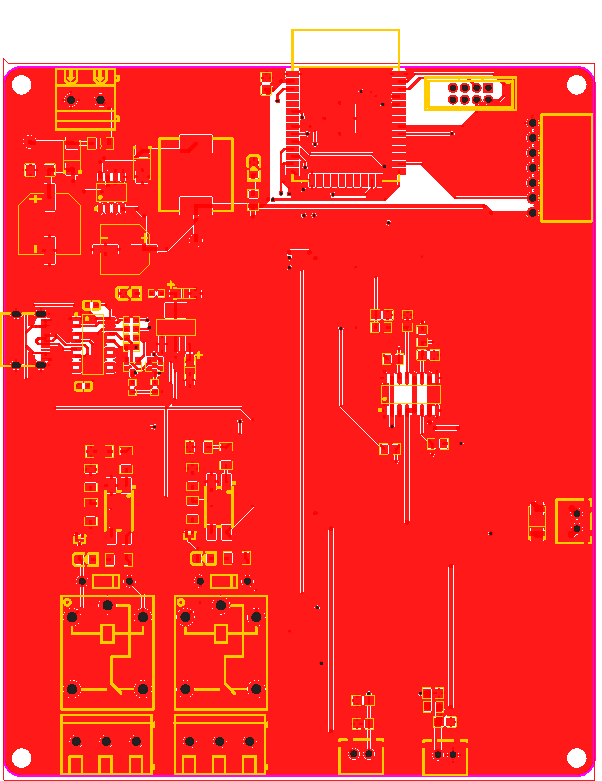
\includegraphics[width=\linewidth]{CHPTRS/CH04_DIS_ELECTRONICO/Fig_Esquematicos/PCB_PCB10_2026-01-30-1.pdf}
  \caption{\textit{Layer} Top de la tarjeta de control.}
  \label{fig:ctrl_top}
\end{subfigure}
\hfill
\begin{subfigure}[t]{0.4\textwidth}
  \centering
  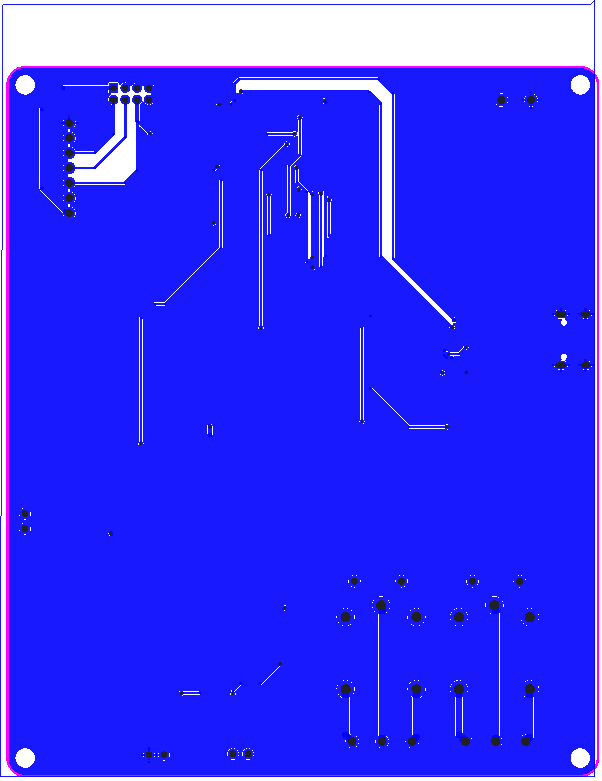
\includegraphics[width=\linewidth]{CHPTRS/CH04_DIS_ELECTRONICO/Fig_Esquematicos/PCB_PCB10_2026-01-30-2.pdf}
  \caption{\textit{Layer} Bottom de la tarjeta de control.}
  \label{fig:ctrl_bottom}
\end{subfigure}
\caption{\textit{Layers} de la tarjeta de control.}
\label{fig:pcb_ctrl_layers}
\end{figure}

\subsection{\textit{Layers} de la tarjeta del sensor}
De igual forma, a continuación se presentan los \textit{layers} de la tarjeta del sensor de efecto Hall: la capa \textit{Top} en la Figura~\ref{fig:sens_top} y la capa \textit{Bottom} en la Figura~\ref{fig:sens_bottom}, presentadas de forma conjunta en la Figura~\ref{fig:pcb_sens_layers}.

\begin{figure}[H]
\centering
\begin{subfigure}[t]{0.4\textwidth}
  \centering
  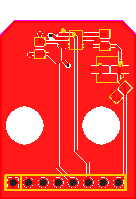
\includegraphics[width=\linewidth]{IMAGENES/DISE_ELEC/DIS_ELEC_09a_LayerSensorTop.pdf}
  \caption{\textit{Layer} Top de la tarjeta del sensor.}
  \label{fig:sens_top}
\end{subfigure}
\hfill
\begin{subfigure}[t]{0.4\textwidth}
  \centering
  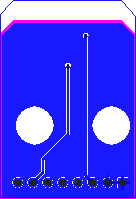
\includegraphics[width=\linewidth]{IMAGENES/DISE_ELEC/DIS_ELEC_09b_LayerSensorBottom.pdf}
  \caption{\textit{Layer} Bottom de la tarjeta del sensor.}
  \label{fig:sens_bottom}
\end{subfigure}
\caption{\textit{Layers} de la tarjeta del sensor.}
\label{fig:pcb_sens_layers}
\end{figure}

\section{Diagramas esquemáticos}
Finalmente, en esta sección se presenta el diagrama de conexiones entre la \ac{PCB} de control y la \ac{PCB} del sensor de efecto \textit{hall}. A continuación, se incluyen los diagramas esquemáticos correspondientes a ambos módulos, los cuales permiten identificar la interconexión de señales, alimentación y comunicaciones necesarias para su integración en el sistema. En la sección siguiente se detallan los criterios de ruteo y el diseño final orientado a su ensamble en el chasis.
